\documentclass[a4paper, 14pt]{extarticle}
\usepackage[russian]{babel}
\usepackage[T1]{fontenc}
\usepackage{fontspec}
\usepackage{indentfirst}
\usepackage{enumitem}
\usepackage{graphicx}
\usepackage[
  left=20mm,
  right=10mm,
  top=20mm,
  bottom=20mm
]{geometry}
\usepackage{parskip}
\usepackage{titlesec}
\usepackage{xurl}
\usepackage{hyperref}
\usepackage{float}
\usepackage[
  figurename=Рисунок,
  labelsep=endash,
]{caption}
\usepackage[outputdir=build, newfloat]{minted}

\hypersetup{
  colorlinks=true,
  linkcolor=black,
  filecolor=blue,
  urlcolor=blue,
}

\renewcommand*{\labelitemi}{---}
\setmainfont{Times New Roman}
\setmonofont{JetBrains Mono}[
  SizeFeatures={Size=11},
]

\newenvironment{code}{\captionsetup{type=listing}}{}
\SetupFloatingEnvironment{listing}{name=Листинг}

\setminted{
  fontsize=\footnotesize,
  frame=lines,
  framesep=2mm,
}

\setlength{\parskip}{6pt}

\setlength{\parindent}{1cm}
\setlist[itemize]{itemsep=0em,topsep=0em,parsep=0em,partopsep=0em,leftmargin=2.0cm,wide}
\setlist[enumerate]{itemsep=0em,topsep=0em,parsep=0em,partopsep=0em,leftmargin=2.0cm,wide}

\renewcommand{\thesection}{\arabic{section}.}
\renewcommand{\thesubsection}{\thesection\arabic{subsection}.}
\renewcommand{\thesubsubsection}{\thesubsection\arabic{subsubsection}.}

\titleformat{\section}{\normalfont\bfseries}{\thesection}{0.5em}{}
\titleformat{\subsection}{\normalfont\bfseries}{\thesubsection}{0.5em}{}

\titleformat*{\section}{\normalfont\bfseries}
\titleformat*{\subsection}{\normalfont\bfseries}

\linespread{1.5}
\renewcommand{\baselinestretch}{1.5}

\begin{document}

\begin{titlepage}
  \vspace{0pt plus2fill}
  \noindent

  \vspace{0pt plus6fill}
  \begin{center}
    Санкт-Петербургский национальный исследовательский университет
    информационных технологий, механики и оптики

    \vspace{0pt plus3fill}

    Факультет инфокоммуникационных технологий

    Направление подготовки 11.03.02

    \vspace{0pt plus2fill}

    Лабораторная работа №1
  \end{center}

  \vspace{0pt plus6fill}
  \begin{flushright}
    Выполнил: \\
    Швалов Даниил Андреевич

    Группа: К33211

    Проверила: \\
    Марченко Елена Вадимовна
  \end{flushright}

  \vspace{0pt plus5fill}
  \begin{center}
    Санкт-Петербург

    2024
  \end{center}
\end{titlepage}

\section{Введение}

\textbf{Цель работы}: разработать веб-приложение, в котором у пользователя будет
возможность загрузить данные из файла.

В данной лабораторной работе необходимо разработать веб-приложение, в котором
пользователь имеет возможность загружать данные из файла в таблицу БД. Файл
находится на локальном компьютере пользователя. Пользователь загружает файл на
сервер, используя веб-интерфейс. Форма интерфейса должна содержать следующие
поля для ввода:
\begin{itemize}
  \item логин;
  \item пароль;
  \item поле для выбора имени файла с данными;
  \item имя SQL-сервера;
  \item имя логина БД;
  \item пароль БД;
  \item имя базы данных;
  \item имя таблицы.
\end{itemize}
После ввода данных пользователь отправляет информацию на сервер.

\newpage

\section{Ход работы}

Для хранения данных, которые загружаются из файла, была выбрана СУБД PostgreSQL.
Данная СУБД поддерживается в языке программирования PHP и не требует
дополнительной установки внешних библиотек для работы с СУБД. Кроме того, СУБД
PostgreSQL является высокопроизводительным решением, обладающим активным
сообществом, большим количеством документации. Данное решение используется
множеством компаний, поскольку оно зарекомендовало себя как надежное и
эффективное хранилище данных.

На рисунке \ref{fig:puml/database.png} изображена схема таблиц базы данных. В
ней представлены две таблицы: <<user\_account>> и <<data>>.

\begin{figure}[H]
  \centering
  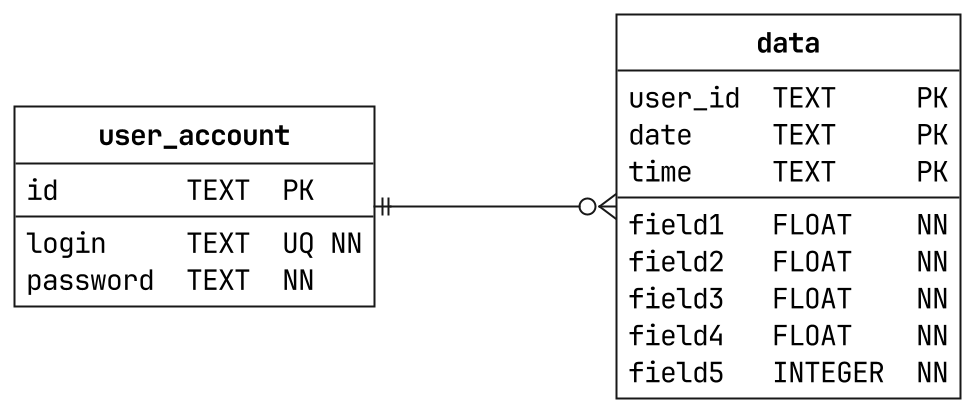
\includegraphics[width=0.8\textwidth]{images/puml/database.png}
  \caption{Схема таблиц базы данных}
  \label{fig:puml/database.png}
\end{figure}

В таблице <<user\_account>> хранится минимально необходимая информация о
пользователе: его идентификатор, логин и пароль. Эти данные используются при
авторизации пользователя.

В таблице <<data>> хранятся данные, загружаемые из файла, а также информация о
пользователе, который загрузил эти данные. В качестве первичного ключа выступает
кортеж из идентификатора пользователя, даты и времени данных. При загрузке
данных, у которых совпадает первичный ключ, данные в таблице обновляются. При
необходимости, вместо <<data>> пользователь может указать другое название
таблицы. Все поля в другой таблице будут идентичными.

При открытии веб-приложения пользователю открывается форма, которая изображена
на рисунке \ref{fig:index.png}. В ней пользователю необходимо указать логин и
пароль от аккаунта, а также приложить файл с данными. В добавок к этому,
пользователь может указать информацию, используемую при подключении к базе
данных.

\begin{figure}[H]
  \centering
  \fbox{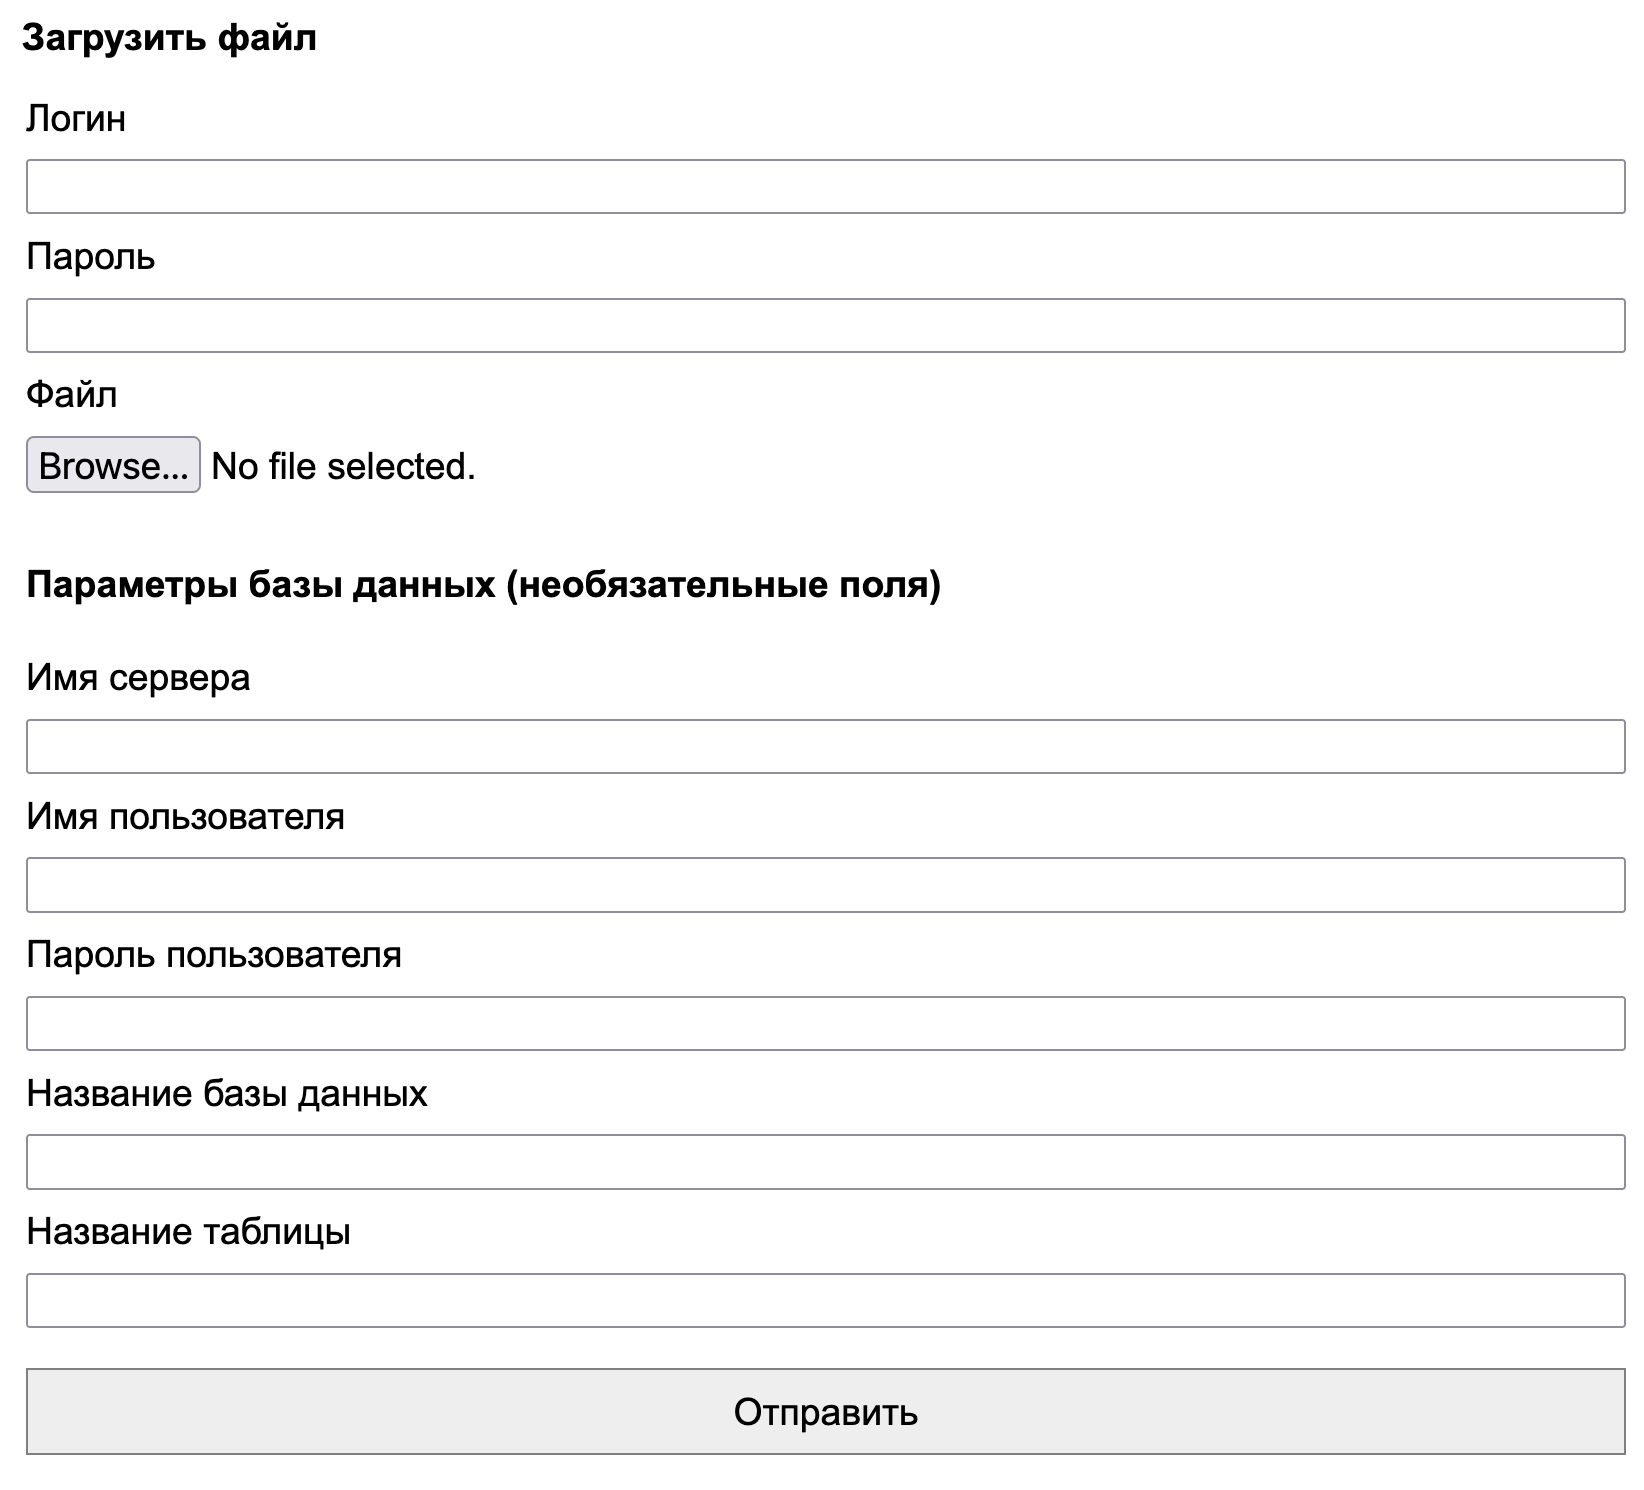
\includegraphics[width=0.8\textwidth]{images/index.png}}
  \caption{Страница с формой отправки файла с данными}
  \label{fig:index.png}
\end{figure}

Если пользователь с данным логином или паролем не будет найден в базе данных
(например, пользователь не существует или пароль не совпал), то будет показана
страница, изображенная на рисунке \ref{fig:user-not-found.png}. Как видно, после
сообщения об ошибке пользователю предлагается вернуться на предыдущую страницу,
и, при необходимости, попробовать снова.

\begin{figure}[H]
  \centering
  \fbox{
\includegraphics[width=0.7\textwidth]{images/user-not-found.png}}
  \caption{Страница, отображаемая в случае, если пользователь не был найден}
  \label{fig:user-not-found.png}
\end{figure}

Если загрузка данных прошла успешно, то пользователю будет показана страница,
изображенная на рисунке \ref{fig:form-success.png}. На ней пользователю
сообщается, что данные были успешно загружены и предлагается вернуться на
главную страницу.

\begin{figure}[H]
  \centering
  \fbox{
\includegraphics[width=0.7\textwidth]{images/form-success.png}}
  \caption{Страница, отображаемая, если данные были успешно загружены}
  \label{fig:form-success.png}
\end{figure}

Пусть пользователь решил загрузить файл со следующими данными:
\begin{minted}{text}
  2017.06.23,07:00,1.1162,1.1167,1.1161,1.1163,108
  2017.06.23,08:00,1.1164,1.1174,1.1163,1.1171,212
  2017.06.23,09:00,1.1172,1.1179,1.1168,1.1175,404
  2017.06.23,10:00,1.1176,1.1187,1.1170,1.1171,423
\end{minted}
Тогда содержимое базы данных будет таким, как изображено на рисунке
\ref{fig:entries.png}. Как видно, все данные из файла были разбиты по полям и
сохранены в базу данных.

\begin{figure}[H]
  \centering
  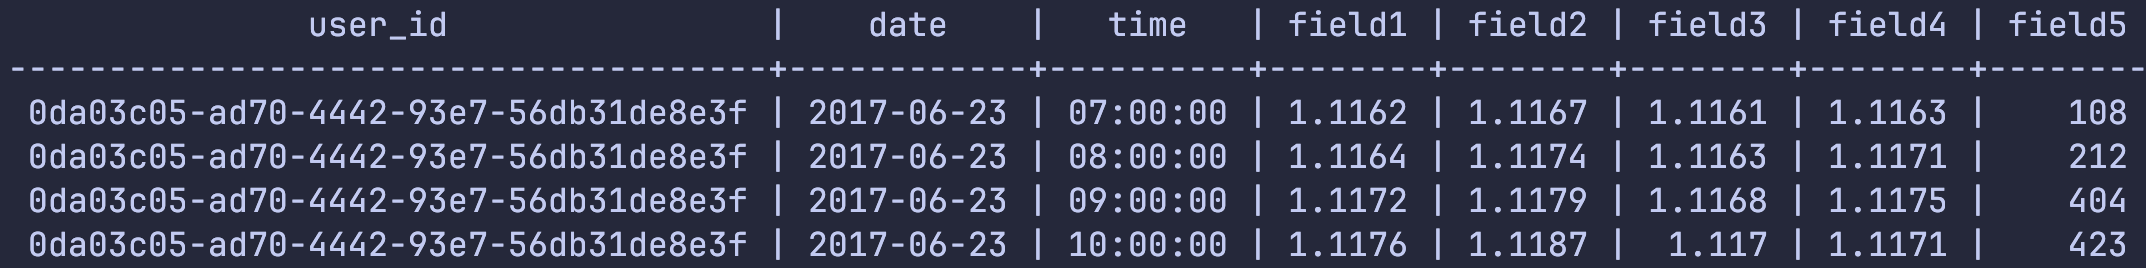
\includegraphics[width=\textwidth]{images/entries.png}
  \caption{Содержимое базы данных после загрузки данных}
  \label{fig:entries.png}
\end{figure}

\newpage

\section{Вывод}

В ходе выполнения лабораторной работы было разработано веб-приложение, в котором
у пользователя есть возможность загрузить данные из файла.

\end{document}
